%!TEX root = ../../dissertation.tex
%%%%%%%%%%%%%%%%%%%%%%%%%%%%%%%%%%%%%%%%%%%%%%%%%%%%%%%%%%%%%%%%%%%%%%%%%%%%%%%
\chapter{Introduction}
\label{chap:intro}


\begin{itemize}

\item ARPANAT and evolutionary process to today's Internet scale
\item outside and inside developments brings new Internet usage (mp3+p2p, bandwidth+codecs -> video, digicams/camcorder); socioeconomic developments of a free speech network;New traffic patterns emerging due to external developments. Digital cameras, new codecs (esp MP3, mpeg4, WebM) -> p2p, Webcams 
\item mobile networks: more of a parallel development to the Internet, always centralized (from the old copper/telephony/circuit switched world)
\item MNs very different to the Internet structures we are used to
\item circuit switched roots, signaling, explicitly NOT a distributed system as compared to Internet, i.e. explicit signaling central controllers
\item Streaming and Multicasting, Multicasting in the Internet in general (only somewhat relevant for live/realtime non-interactive stuff)
\item  network intelligence at the end nodes
\item --> end-to-end violations: ECN? only signaling, decision is e2e, same category as indirect TCP congestion control signaling (through loss) from the network; NAT, Firewalls?
\item content agnosticism: we do not know what applications the future will bring, so we do not make any assumptions
\item HTTP; ``The Web adopts relatively simple technologies with sufficient scalability efficiency and utility'' \cite{W3Arch}
\item Why HTTP streaming? Generalization of HTTP streaming (reliable transport, control shift to the client); Less control, more effective; Why global \gls{QoS} control doesn't work
\item \gls{LTE}, \gls{EPC}, Core network tunneling concepts, bottlenecks in the access and the core, \gls{LTE} network model
\item Improvements to congestion control for mobile streaming
\item Influence of L1/2/3 layer protocols and mechanisms (IPv4/6, tunneling, ethernet vs RLC/RRC/NAS, ...) ; what works better with it? compare, model and measure
\item \gls{QoE} metrics, \gls{MOS}, stalling time and buffering models, subjective and objective testing
\item http://www.ipjforum.org/?p=926 Vint Cerf looking forward

\item Data-mining of network trace data from mobile networks.
\item Investigation of mobility awareness and prediction techniques ("unassisted mobility")

\end{itemize}

%% new thesis stuff
Packet Switching, the process of chunking information into smaller bits, labeling it and transmitting it independently, was first described by Paul Baran in the 1960s\cite{baran1964distributed}. This changed communication a lot and provided one of the foundations for the emergence of the Internet. 

The original usage intent was mostly limited to remotely logging into and communicating with mainframe computers and transferring files supported by the emergence of new multiuser and multitasking operating systems, especially including the release of UNIX in 1969.\todo{needs references}

From these early times countless other services and applications emerged. Today, the Internet is by used hundreds of millions of people, touching almost every aspect of daily life. The creation of the World Wide Web -- begun by Tim Berners-Lee in 1989\todo{reference} -- brought an easily accessible ``user interface'' to the Internet and made adoption for the masses much easier. Today, almost any form of application is available through the Web as a combination of \gls{HTML}, \gls{CSS}, and JavaScript and can be accessed by just opening a Web browser.

But as is the case with many technological fields, the Internet's development was also closely entangled with other advancements. Take the huge Internet music wave beginning in 1999 as an example. It may have been started by the creation of Napster, the first peer-to-peer file sharing service. However, without the large improvements in audio compression -- namely MP3 -- a few years before, including computers that could handle decompression as well as compression and increasing Internet access bandwidth (and fixed service fees) , this would not have been possible. Similarly, YouTube could not have existed without a wide spread of digital camcorders and many other devices with recording capability, good video compression codes, and an even further increase in access bandwidths.
 For every leap in bandwidth new services sprung to life fueling the users' demand for further capacity increases. 

% content agnosticism: we do not know what applications the future will bring, so we do not make any assumptions

Several factors contributed to the quick acceptance of the Internet. First and foremost no assumptions are made on the transported content, or content agnosticism. The original idea is to treat every packet, every participating node the same and do not make any assumptions on specific applications. This provides a level playing field for every contender wanting to offer services. This is upheld by the second driving concept, the ``End-to-End Principle'', \cite{saltzer1984end2end} stating:

\begin{quote}
``The function in question can completely and correctly be implemented only with the knowledge and help of the application standing at the endpoints of the communications system. Therefore, providing that questioned function as a feature of the communication system itself is not possible. [...]''
\end{quote}

End-to-End means that any functionality, meaning services or applications, should only be implemented at the two endpoints of a transmission not somewhere in between. Tuning the network to specific applications and implementing functions inside the network, will always only be valid for existing and narrow use cases and cannot support future developments.

During the past decades this has often been discussed  \cite{bhattacharjee1997active, blumenthal2001rethinking, isenberg1997rise, lemley2000end} but is still being upheld for the most part for good reason. \todo{probably should clarify the good reason}. This is in contrast to the way telephone networks and their operating companies historically worked. These networks are based on circuit switching and access as well as content (namely voice calls) and procedures are tightly controlled by the operator.
%\\

%%%%%%%%%%%%%%%%%%%%%%%%%%%%%%%%%%%%%%%%%%%%%%%%%%%%%%%%%%%%%%%%%%%%%%%%%%%%%%%%
\section{Video and the Internet}

\begin{figure}[htbp]
    \centering
    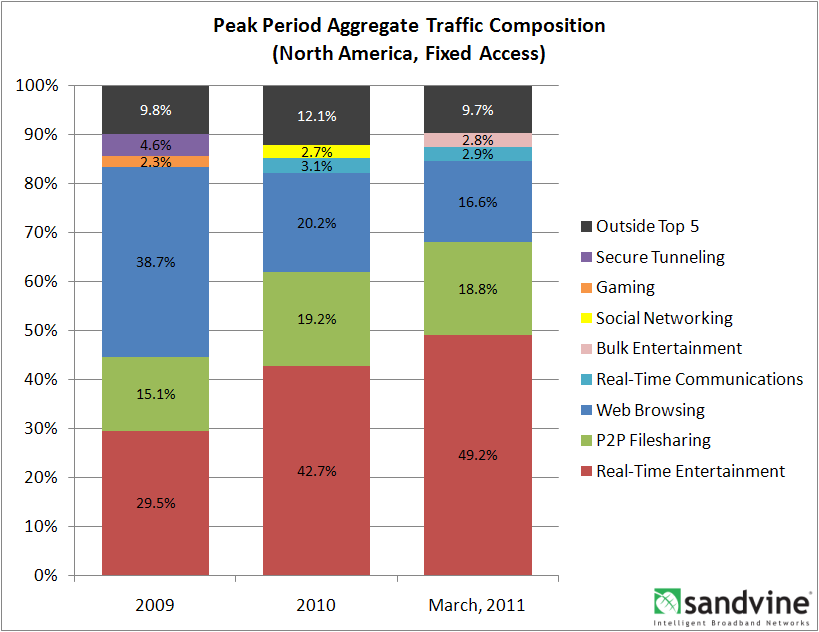
\includegraphics[width=0.8\textwidth]{images/netvine.png}
    \caption{Netvine, North American peak traffic (Source: \cite{sandvine_spring2011,sandvine_spring2013}).}
    \label{c1:fig:traffic_netvine}
\end{figure}

\begin{figure}[htbp]
    \centering
    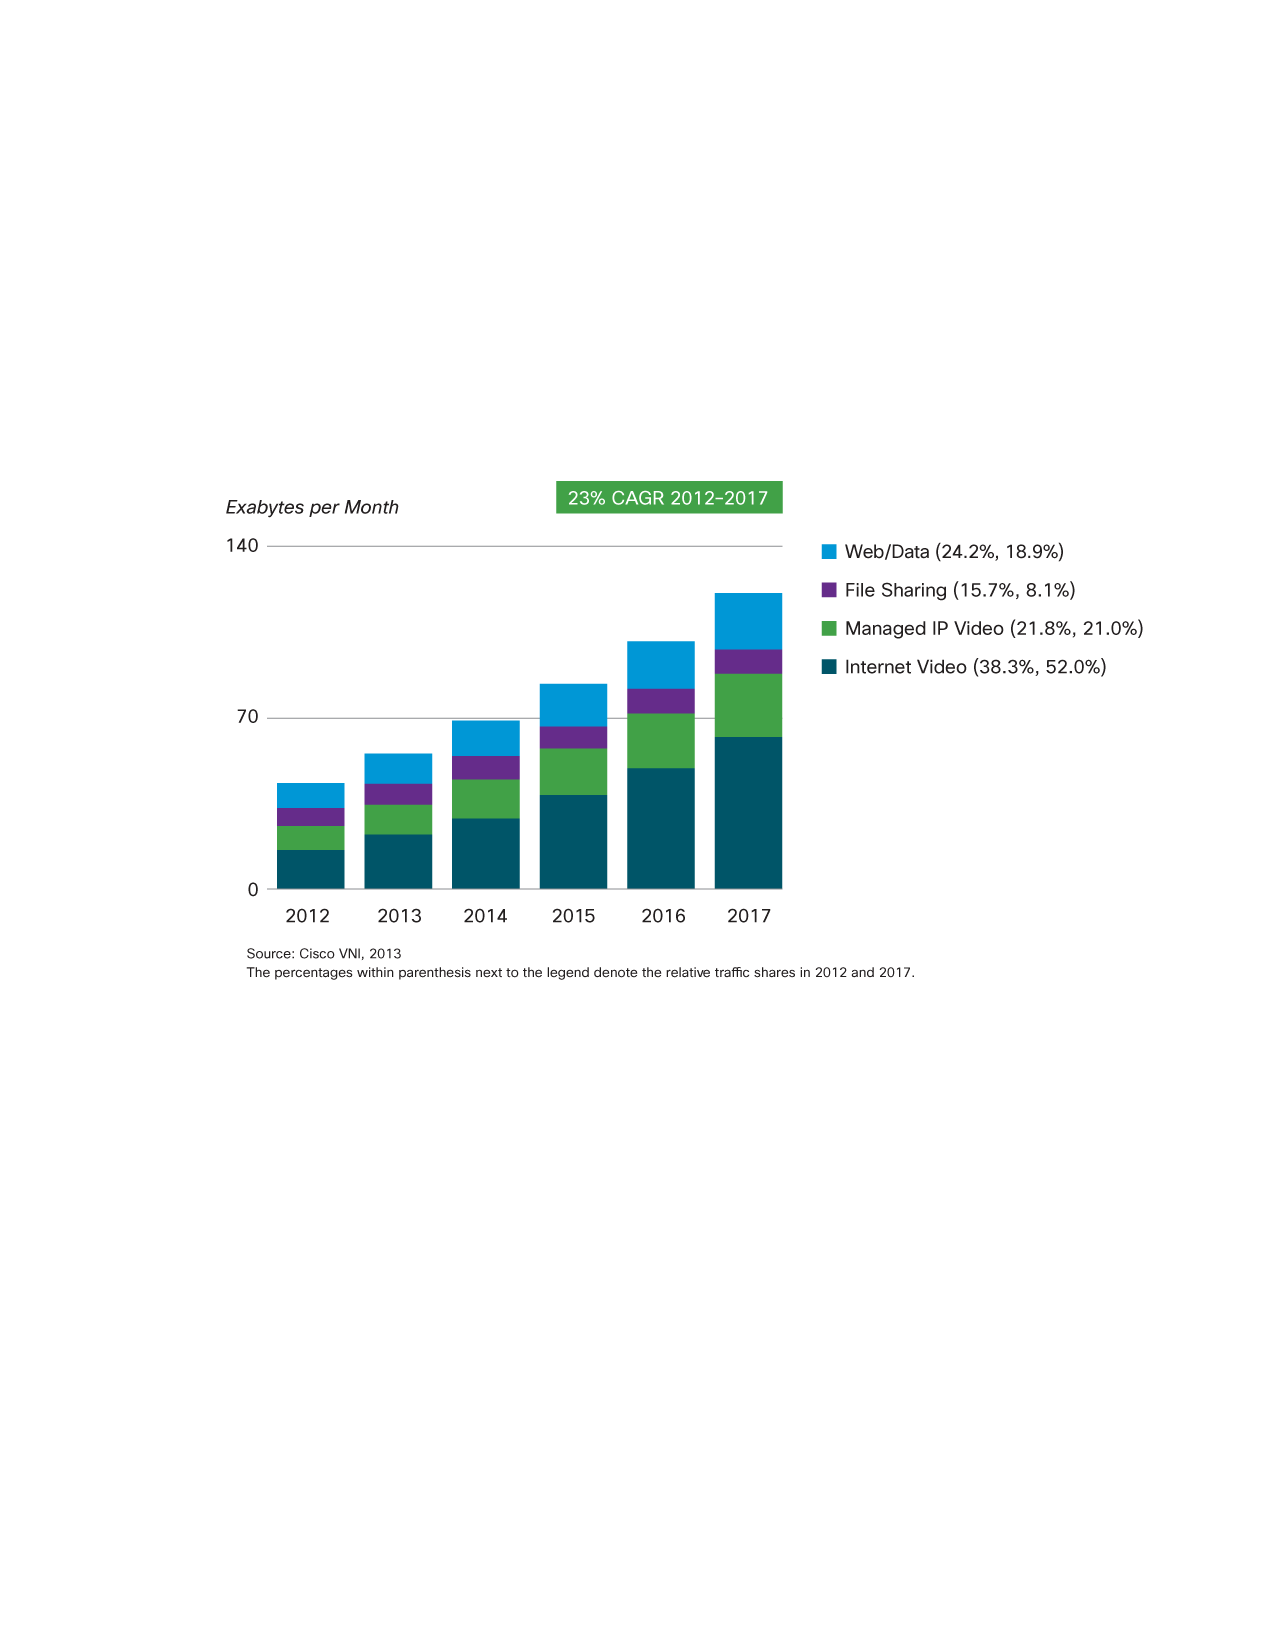
\includegraphics[width=0.8\textwidth]{images/VNI_Hyperconnectivity_WP.pdf}
    \caption{Cisco, global consumer Internet traffic prediction (Source: \cite{cisco2013VNI}).}
    \label{c1:fig:traffic_cisco}
\end{figure}

The total volume of Internet traffic has been rising exponentially for many years. The composition of today's traffic is manifold, but one of the largest contributing factors is arguably video (take a look at Figures~\ref{c1:fig:traffic_netvine} and \ref{c1:fig:traffic_cisco}). Studies predicting the development of the Internet's traffic also tell of the large influence of video in the near future. The two main sources for this video are YouTube\footnote{\url{https://www.youtube.com}} and, in countries where its available, Netflix\footnote{\url{https://www.netflix.com}}, and even newer services like the live-streaming site Twitch\footnote{\url{http://twitch.tv}} acting as runner-up.

Despite not wanting to tune the network to video, it is still very important to understand the dynamics happening around this type of traffic there. With a traffic portion this large any events or behavior specific to this portion will also have a huge impact on the total network.
Transporting this video -- or rather ``streaming'' as in watching the video while it's still being transmitted -- -- integrating themselves much better into the current Web ecosystem --  in the Internet has again become a topic of hot discussions. There are long-standing application layer protocols for exactly this use case. \gls{RTP}, as the most prominent, has been described as early as 1996 \cite{rfc1889}. It is well described in standard educational literature and specifics to it are still being researched and improved on. Interestingly however, it is practically not being used at all in the current updraft of video traffic. \todo{explain the reason (Web-relationship, tcp basis, firewalls, walled gardens, ...)either here or in a later chapter}
Instead, new approaches have been thought out, integrating themselves much better into the current Web ecosystem.
And they are using completely different modes of transportation and control. Streaming, and media transport in general, is also not only relevant for the purpose of watching videos, there are many more fields of use with similar requirements. Becoming popular in the last years is the so-called Cloud Gaming: Running virtualized video games on large racks and streaming just the video output to the clients with all the user input handled by the server, putting a huge emphasize on achieving low latency.\footnote{Select works overviewing this thematic complex are, e.g., \cite{4795441,wang2009modeling,jarschel2011cloudevaluation,ct2010wolken}.}
Investigating the implications coming with these new streaming protocols will be the first task of this thesis.
%\\

%%%%%%%%%%%%%%%%%%%%%%%%%%%%%%%%%%%%%%%%%%%%%%%%%%%%%%%%%%%%%%%%%%%%%%%%%%%%%%%%
\section{The Network Below}

Looking back to the actual networks, we also see lots of progress in the past. Despite their rapid evolution, mobile networks, however, still carry much heritage from their circuit switching roots. \footnote{For an historical overview refer to \url{https://en.wikipedia.org/wiki/History_of_mobile_phones}. \todo{should remove wikipedia}}
Starting in the 1950s with early analog predecessors like the German ``A-Netz'' and first generation cellular structured networks in the eighties, mobile telephony entered the fully digital world with the European \gls{GSM} and competing \gls{CDMA}-based technologies around the year 1991. This was similar to the development in the \gls{POTS} with its shift away from the analog roots to digital circuit switching technologies like \gls{ISDN}.

Because of its huge success \gls{GSM} and its packet-switching extension \gls{GPRS} was used as a blueprint for the following mobile network standard evolutions resulting in \gls{UMTS} (including \gls{HSPA} and \gls{HSPA+}), today's \gls{LTE} and even the upcoming \gls{LTE} Advanced. Through this heritage, many network elements and protocol have hardly changed since the beginning and are still strongly connection orientated with a strong tendency to signaling and statefulness.
This creates a wide range of problems which have only begun to show up in recent years due to the large influx of new user and usage scenarios, creating traffic patterns unheard of a few years ago and overwhelming the network's control plane structures. 

Traffic in cellular networks follows a development similar to that of the Internet as a whole. Through the advent of affordable high performance smartphones, a thriving mobile application ecosystems, and (relatively) fast access technologies many are now using their phones as the primary device for interacting with the Internet. Video, too, has here become one of the largest contributors of cellular traffic. 

However, heavy traffic on a stateful network poses unique challenges to the performance, the design, and dimensioning of network protocols. This gets even more complicated by the circumstance, that operators and vendors usually regard any details on mobile networks equipment as closely kept trade secrets Thus, little is known of the exact make-up of these networks as they are closely guarded secrets of the operator.

This presents us with the second task of this thesis.



%%%%%%%%%%%%%%%%%%%%%%%%%%%%%%%%%%%%%%%%%%%%%%%%%%%%%%%%%%%%%%%%%%%%%%%%%%%%%%%%
\section{Research Methods and Approaches}

As is the case with any scientific endeavor, this work is based on a specific set of tools and knowledge of many years of prior research. Measuring, evaluating and modeling is standard practice in many fields. Therefore, many tools  are available to tackle problems, but one still has to choose the most fitting ones for a given problem.


\begin{figure}[htbp]
    \centering
    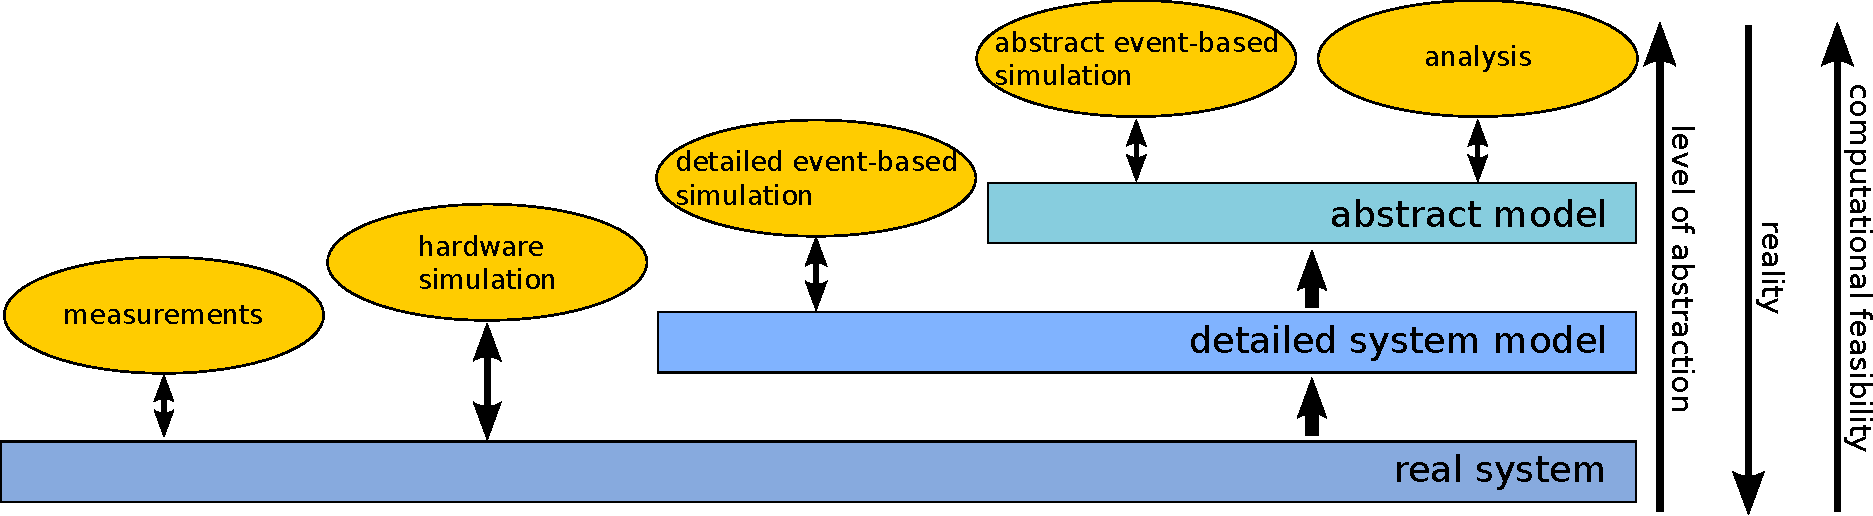
\includegraphics[width=1.0\textwidth]{images/apparatus-new.pdf}
    \caption{Methodical solution spaces and apparatus comparison.}
    \label{c1:fig:appcomp}
\end{figure}

Figure~\ref{c1:fig:appcomp} attempts to categorize all tools available to a performance analyst, with their corresponding level of detail and abstraction.

The most precise results will always be achieved through actual measurements of the actual system under scrutiny. This will give a point of reference and can be used to validate the accuracy of other methods. But it also comes with a hefty price of huge amounts of data to process and understand. With such measurements at hand, one can now start to make sense of this data and extract the relevant features observed in this process.

Aside from measurements on implementations there are three further possible approaches to widen the scope: emulation, simulation, and mathematical analysis or analytical models.  An emulation tries to resemble implemented functionality as closely as possible with the cost of high complexity. While there are many forms of emulation, relevant to our research interests is just the so-called network emulator. Instead of having a real network, parts of it are substituted with emulating hardware or software that treats transmissions according to properties from the actual network. Most typically these properties are the transmission bandwidth, loss, and latency (and variation over time thereof).
But emulations always just replace parts of the actual system and therefore its capability to scale is limited.

This is where simulations come into play, implementing all internal and external functionality, including the physical nodes and the network in software. A typical \gls{DES} can have subtle functional differences but can be scaled almost indefinitely limited only by the available processing time. 

Prior to any simulation or emulation and following every measurement on a system is of course the mathematical analysis of existing data. Through this models are built abstracting the system the data is gathered from. With every iteration the model can be refined and new hypotheses formed.
A mathematical analysis, for example using queuing theory and stochastic models, can then further broaden the understanding of the system.


\todo{mention here? Application of queuing theory, modeling the system through arrival processes, service time distributions and a number of servers and waiting places.}


%%%%%%%%%%%%%%%%%%%%%%%%%%%%%%%%%%%%%%%%%%%%%%%%%%%%%%%%%%%%%%%%%%%%%%%%%%%%%%%%
\section{Lines of Research and Goals}

With these tools at hand, this thesis will follow in most parts two mostly independent lines of research.

The first line will be a thorough investigation of current video streaming mechanisms and services facilitating them. All of the investigated streaming ``protocols'' are comparatively young and similar. 

Protocol is put in parentheses for a reason here. Many of the approaches are not protocols in the classical sense. They do not follow a specification of any standards body, be it \gls{ISO}, \gls{ITU} or the \gls{IETF}. Neither do they show much distinction in the way the use the network and transport video as they simply rely on normal Web protocols. Rather, much of their differences stems just from the behavior of the actual application. The way how it requests and retrieve the data and displays the video, including its reaction to unwanted events, e.g. having insufficient data in the playback buffer. 
Surprisingly, even just with these rather simple rules, applications can still distinguish themselves from one another. Making the right decisions to events can greatly influence the quality of the video playback. 

During the investigation we created a model describing all the common elements in the streaming process. With such a model at hand and in knowledge of the structure and similarities of the applications, one can do many things. Through a performance analysis they can be compared to each other. Interrelations to the network's transport layer and other influences of the network on streaming could be uncovered. This especially includes mobile networks where many assumptions made for wired networks do not hold anymore. One quick example is the circumstance, that the network layer and all layers above generally do not experience any packet loss in a cellular network. Any loss is treated by the mobile layers, albeit with other side effects on the upper layers. For example, they will experience intermittent times of extremely high latency.
This leads to the question, on which kind of information from the network a streaming application could and should depend, or even if there are any actual requirements for streaming.

Gathering this kind of information can result in a better understanding of the quantitative attributes related to these new forms of streaming. The results can be used as an analytical and testing tool for improving the protocols or even lead to different approaches. Furthermore, the thesis aims to provide methods for helping all parties involved in media streaming decide which protocols and methods to choose and which are best suited for specific scenarios.
\\

The second line of research will deal mostly with the described oddities of cellular networks. Through exploration of currently existing networks and architectural specifications data is gathered. This data allows to draw some very interesting conclusion regarding states and signaling in these cellular nets and possible load caused by it. Those conclusions and further evaluations also lead to a model for the core network, abstractly describing the control plane. This will ultimately help to improve the planning and dimensioning of networks, even influence future specification iterations to reduce their fixation on signaling.


For the third and final field of research an attempt is made to bridge both of these lines. With the increasing prevalence of video streaming in mobile networks, it is important to understand the relationship between these two. Here, this will follow mostly a theoretical approach, with descriptions to protocol drafts dealing with these kinds of issues. 

Measuring mobile networks is always rather complicated, with a vast number of variables to keep track of and control. To give an example, just think of the movement patterns of mobile devices and the impact this has on handovers between cells as well as the signal strength, and therefore also on packet loss, and, e.g., the video quality.
 To improve this situation, two methods are explored. Reducing the number of variables -- but thus also the level of detail -- can be easily achieved using network simulation or emulation. This has also the added advantage of having easy access to all nodes in the (simulated) network. The simulator can then be combined with either traffic from real applications, or the applications under scrutiny can also be simulated.
 If simulating is out of the question and real-world mobile phone measurements are to be conducted, maybe even as part of a measurement testbed spanning many devices, the phone's state needs to be recorded as precisely as possible. Thankfully, today's mobile phone have a multitude of sensors and information sources available, which will be exploited in the measurement approach present second.
 Lastly, with the knowledge from all of the investigations, a proposal for a new paradigm managing networking application traffic -- especially in cellular networks where mobility matters -- is given.



%%%%%%%%%%%%%%%%%%%%%%%%%%%%%%%%%%%%%%%%%%%%%%%%%%%%%%%%%%%%%%%%%%%%%%%%%%%%%%%%
\section{Main Contributions and Structure}

Following these research lines, several contributions are made, which will be broken down into three major chapters.

To introduce to the video streaming investigations, covered in Chapter~\ref{chap:streaming}, at first the protocols and techniques, that have been used in the past, will be described in Section~\ref{c3:background}. This then leads, to a broad survey of current protocols. A subset of them will serve as the basis for the presented \gls{TCP} streaming model. Furthermore, to be able to work with the model, an evaluation metric is required, one will be created in Section~\ref{c3:metrics}, as the selection of existing metrics does not fulfill the needs of our model. Now that both metric and model are ready, a measurement study using an emulation approach is conducted in Section~\ref{c3:measurements}, investigating the performance of an actual video streaming service with the help of the model under the influence of varying network conditions.

The facets of mobile networks, and especially the core network, are researched in Chapter~\ref{chap:mobilenets}. As the amount of specifications as well as architecture, procedure, and protocol details is vast, the first section (\ref{c4:background}) attempts to put all the basics together. 

The tackled protocols, systems, and mechanisms are described in Section X. Section Y details the methods that are and are planned to be used for the research. The final section gives a rough estimation on the thesis' schedule. The remainder of the chapter uses data from a passive measurement campaign at a mobile operator. Section~\ref{c4:methodology} describes how the data was acquired and how this data can be interpreted. With this foundation laid out, the actual goal of the investigations will now be defined in Section~\ref{c4:loaddefinition}: an alternative definition and investigation of load in a mobile network, based the control plane and not just the user plane. This goal is pursued throughout the exploratory evaluations of the dataset in Section~\ref{c4:evaluations}. Learning from the data novel load models are then formulated in \ref{c4:modeling} and thoroughly tested using a queuing simulation. With these models mobile network operators can better dimension and plan their networks according to control plane load and not just to accommodate user traffic.


Finally, some thoughts and approaches to study and improve traffic -- especially video streaming traffic -- in mobile networks are collected in Chapter~\ref{chap:mobilestreaming}.  As mobile devices depend on a lot more variables (with mobility being the most prominent) than devices with fixed Internet access, any measurement needs to keep track of these. Section~\ref{c5:sensorium} presents our approach to tackling this.
Section~\ref{c5:mobilestreamingtestbed} adapts the earlier described streaming measurement model to work with a mobile network simulation and emulation.
And finally, Section~\ref{c5:crosslayerhinting} presents a model to improve any traffic that can be broken down into segments, .e.g. adaptive streaming or Web traffic, by providing cross-layer \glspl{API}.
\todo{add the chapter specifics, when they are fleshed out}

%% <-- %% WIP


%The methods can all be used to define and explore solution spaces and are therefore important tools in understanding the problem. A fitting combination of these tools has to be found to advance the research. Our initial approach is to investigate existing streaming services, YouTube \cite{metzger2011delivery,mokmeasuring} and, e.g., video libraries of broadcast stations for simple HTTP streaming. A suitable candidate for measuring adaptive streaming still needs to be found as some candidate services apply regional restrictions. There are several reference applications available that implement different standardization approaches. These can be used to either directly measure the performance or to setup an emulation model based on their specifications.


% \begin{figure}[htbp]
%     \centering
%     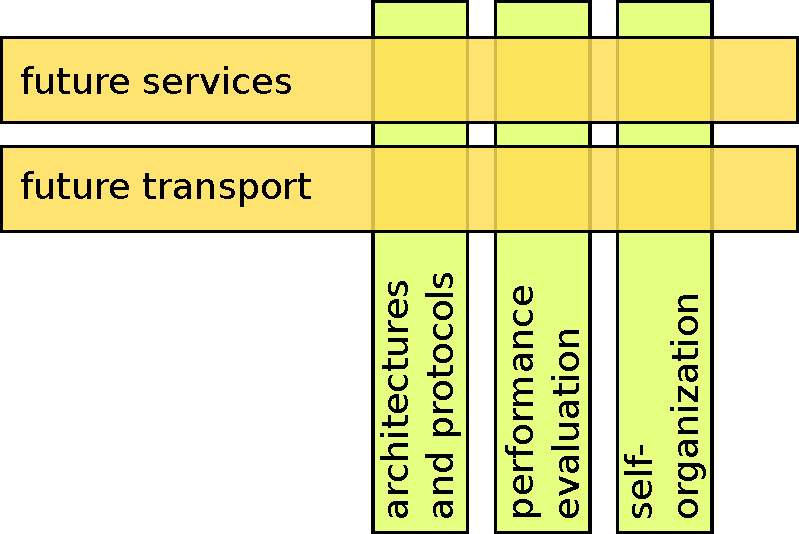
\includegraphics[width=0.7\textwidth]{images/hv-topics-new.pdf}
%     \caption{Technical solution spaces to the problem layers.}
%     \label{c1:fig:hv-topics}
% \end{figure}

%This can put pressure on the overly complex cellular network structures. The radio transmissions have only access to a limited radio frequency spectrum that, moreover, has to be shared with any other phone user in the same cell. But there is also deemed to be significant pressure on the traffic management mechanisms of the mobile core networks backing up and aggregating the numerous radio cells of an operator. 


%As discussed, the core problems are layered into services and transport. Technologically, to solve the tasks of video streaming, one can approach these  in three different ways.

%The first is to dissect the involved protocols and architectures and break them down into their functional and methodical components. This will result in an improved understanding on the manner and process of their implementation. These components serve as building blocks for generalized models that abstracts the problem space from the actual implementation. The model will be defined by a set of parameters. To explore viable parameter ranges performance evaluation methods will be facilitated.

%Secondly, using performance evaluation a system is methodically tested to the outcome of determining the influence of the system's parameters on a set of performance metrics. The parameters can be categorized into system intrinsic parameters, describing behavior only relevant and observable inside the system, and external parameters. In communication networks a good example for external parameters are the network \gls{QoS} parameters including latency, loss, jitter, and bandwidth capacity. Identifying fitting metrics for the measurement is a challenge. They can be either subjective or objective. The former are called \gls{QoE} metrics. They can only be measured by conducting empirical user studies and questionnaires and are mapped to a \gls{MOS}. Extensive work has already been done to define baseline references for QoE metrics. Using these, one can directly translate objectively measurable outcomes into \gls{QoE} metrics. However, these mappings may need to be adjusted to be able to handle stalling as the main source of quality loss. Examples for measuring subjective quality are available in \cite{gustafsson2008measuring, ketyko2010qoe}. Finally, one could employ methods of self-organization to try to reach improvements over conventional network setups.